%%%%%%%%%%%%%%%%%%%%%%%%%%%%%%%%%%%%%%%%%%%%%%%%%%%%%%%%%%%%%%%%%%%%%%%%%%%%%%%%
%2345678901234567890123456789012345678901234567890123456789012345678901234567890
%        1         2         3         4         5         6         7         8

\documentclass[letterpaper, 12 pt]{article}  % Comment this line out
%\documentclass{article}  % Comment this line out
                                                          % if you need a4paper
%\documentclass[a4paper, 10pt, conference]{ieeeconf}      % Use this line for a4

                                                          % paper
\usepackage{amsmath}
\usepackage{array}
\usepackage[samesize]{cancel}
\usepackage{subfigure}
\usepackage{stfloats}
% The following packages can be found on http:\\www.ctan.org
\usepackage{graphics} % for pdf, bitmapped graphics files
\usepackage{epsfig} % for postscript graphics files
%\usepackage{mathptmx} % assumes new font selection scheme installed
%\usepackage{times} % assumes new font selection scheme installed
%\usepackage{amsmath} % assumes amsmath package installed
%\usepackage{amssymb}  % assumes amsmath package installed



\title{\LARGE \bf
ME 532 Project Proposal
%Bandwidth Limitations of Force/Torque Controlled Actuators
%Actuators and You!\\
}

\author{ \parbox{3 in}{\centering Kevin Kemper}}

%\author{Kevin Kemper, Devin Koepl and Jonathan Hurst% <-this % stops a space
%\thanks{This work was not supported by any organization}% <-this % stops a space

%\thanks{P. Misra is with the Department of Electrical Engineering, Wright State University,
%        Dayton, OH 45435, USA
%        {\tt\small pmisra@cs.wright.edu}}%
%}


\begin{document}

\begin{flushright}
Kevin Kemper
\end{flushright}

%\maketitle
\thispagestyle{empty}
\pagestyle{empty}

%%%%%%%%%%%%%%%%%%%%%%%%%%%%%%%%%%%%%%%%%%%%%%%%%%%%%%%%%%%%%%%%%%%%%%%%%%%%%%%%
%\begin{abstract}



%\end{abstract}


%%%%%%%%%%%%%%%%%%%%%%%%%%%%%%%%%%%%%%%%%%%%%%%%%%%%%%%%%%%%%%%%%%%%%%%%%%%%%%%%
\section{ME 532 Project Proposal}


The goal of this work is to develop control laws that will stop a monopod robot (fig. \ref{fig:robot})
dropped from some height in minimum time.  Understanding this problem is a stepping
stone to developing 2-DOF controllers that will allow our running robot to suddenly stop.
It will also facilitate the investigation of how spring values in the robot affect
the performance of this system so that we can intelligently decide on the physical
components.

The basic model of the system (fig. \ref{fig:SEDA}) for a single degree of freedom.
In this problem the robot is constrained to only allow vertical motion.  The actual
robot has two collinear motors at roughly the center of mass.  By activating them
with equal and opposite torques we can remove any body reactions and vector the
toe force directly in one dimension through the COM.

%%%%%%%%%%%%%%%%%%%%%%%%%%%%%%%%%%%%%%%%%%%%%%%%%%%%%%%%%%%%%%%%%%%%%%%%%%%%%%%%
\section{System model}
	
	\begin{figure}[h]
		\centering
		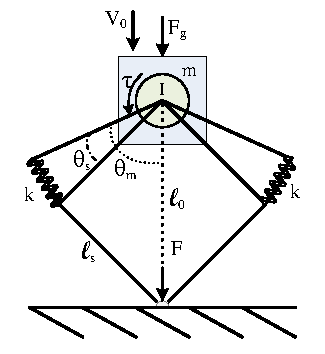
\includegraphics[scale=1.5]{./images/SEDA_atrias.pdf}
		\caption{	The basic model of the system for a single degree of freedom.
					In this problem the robot is constrained to only allow vertical
					motion.}
		\label{fig:SEDA}
	\end{figure}
	
%%%%%%%%%%%%%%%%%%%%%%%%%%%%

	\begin{center}
	\textbf{Variables:}
	\[
	\begin{array}{c|l|l}
	\tau(t) & \textrm{Motor force} & N\cdot m\\
	 & \\
	\theta_{m}(t) & \textrm{Motor position} & rad\\
	\theta_{s}(t) & \textrm{Spring deflection} & rad\end{array}\]
	\textbf{Constants:}\[
	\begin{array}{c|l|l}
	k & \textrm{Spring constant}\\
	 & \\
	m & \textrm{Body mass} & kg\\
	I & \textrm{Motor/tranmission inertia} & kg\\
	\tau_{limit} & \textrm{Motor torque limit} & N\cdot m\\
	\ell_{0} & \text{Initial length} & m\\
	\ell_{s} & \text{Segment length} & m\\
	F_{g} & \text{Gravity} & N\end{array}\]

	\par
	\end{center}

	\[
	\theta=\theta_{M}+\theta_{S}\]
	\begin{eqnarray*}
	\ell_{0} & = & 2\ell_{S}\cos\theta_{M}\\
	\frac{\ell_{0}}{2\ell_{S}} & = & \cos\theta_{M}\\
	\theta_{M} & = & \arccos\left(\frac{\ell_{0}}{2\ell_{S}}\right)\end{eqnarray*}
	\begin{eqnarray*}
	\ell & = & 2\ell_{S}\cos\left(\theta_{M}+\theta_{S}\right)\\
	\frac{\ell}{2\ell_{S}} & = & \cos\left(\theta_{M}+\theta_{S}\right)\\
	\theta_{M}+\theta_{S} & = & \arccos\left(\frac{\ell}{2\ell_{S}}\right)\\
	\theta_{S} & = & \arccos\left(\frac{\ell}{2\ell_{S}}\right)-\theta_{M}\\
	\theta_{S} & = & \arccos\left(\frac{\ell}{2\ell_{S}}\right)-\arccos\left(\frac{\ell_{0}}{2\ell_{S}}\right)\end{eqnarray*}
	\[
	\tau=k\theta_{S}\]
	\begin{eqnarray*}
	F & = & \frac{2\tau\sin\left(\theta_{M}+\theta_{S}\right)}{\ell_{S}}\\
	F & = & \frac{2k\theta_{S}\sin\left(\theta_{M}+\theta_{S}\right)}{\ell_{S}}\end{eqnarray*}


	Pluggin in $\theta_{S}$ we have:\begin{eqnarray*}
	F & = & \frac{2k\left(\arccos\left(\frac{\ell}{2\ell_{S}}\right)-\arccos\left(\frac{\ell_{0}}{2\ell_{S}}\right)\right)\sin\left(\theta_{M}+\arccos\left(\frac{\ell}{2\ell_{S}}\right)-\theta_{M}\right)}{\ell_{S}}\\
	F & = & \frac{2k\left(\arccos\left(\frac{\ell}{2\ell_{S}}\right)-\arccos\left(\frac{\ell_{0}}{2\ell_{S}}\right)\right)\sin\left(\arccos\left(\frac{\ell}{2\ell_{S}}\right)\right)}{\ell_{S}}\end{eqnarray*}
	Using the trigonometric identity:\begin{eqnarray*}
	\sin\left(\arccos x\right) & = & \sqrt{1-x^{2}}\end{eqnarray*}
	We have:\begin{eqnarray}
	F & = & \frac{2k\sqrt{1-\frac{\ell^{2}}{4\ell_{S}^{2}}}\left(\arccos\left(\frac{\ell}{2\ell_{S}}\right)-\arccos\left(\frac{\ell_{0}}{2\ell_{S}}\right)\right)}{\ell_{S}} \label{eq:fk}
	\end{eqnarray}
	
%%%%%%%%%%%%%%%%%%%%%%%%%%%%

	From this calculation we can show that the spring function is nonlinear.  We
	can now use this derivation to to abstract the system into a model composed of
	the motor inertia (represented as a mass) connected to the body through the spring
	defined by equation (\ref{eq:fk}).

	\begin{figure}[h]
		\centering
		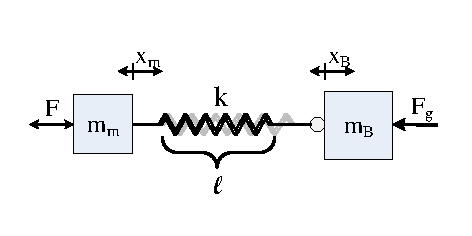
\includegraphics[scale=1.2]{./images/SEDA_atrias_simple.pdf}
		\caption{	Abstracted model of the robot.}
		\label{fig:SEDA}
	\end{figure}


	\begin{figure}[h]
		\centering
		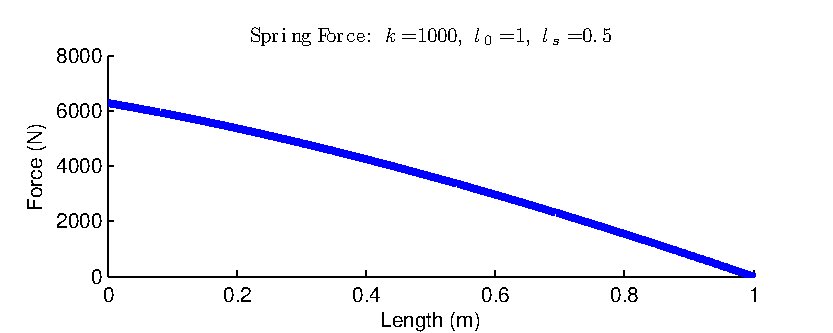
\includegraphics[scale=1]{./images/SpringFunction.pdf}
		\caption{	Spring force as a function of leg length.}
		\label{fig:SEDA}
	\end{figure}


%%%%%%%%%%%%%%%%%%%%%%%%%%%%%%%%%%%%%%%%%%%%%%%%%%%%%%%%%%%%%%%%%%%%%%%%%%%%%%%%
\section{System dynamics}


	Spring length as a function of motor mass and body mass positions:
	\[
	\ell=\ell_{0}-x_{m}+x_{B}
	\]
	Substitute into (\ref{eq:fk}):
	\begin{eqnarray*}
	F_{k} & = & \frac{2k\sqrt{1-\frac{\left(\ell_{0}-x_{m}+x_{B}\right)^{2}}{4\ell_{S}^{2}}}\left(\arccos\left(\frac{\left(\ell_{0}-x_{m}+x_{B}\right)}{2\ell_{S}}\right)-\arccos\left(\frac{\ell_{0}}{2\ell_{S}}\right)\right)}{\ell_{S}}
	\end{eqnarray*}
	\\
	\textbf{Note:} spring can only be in compression!


	\begin{itemize}
		\item System 1 (actuator side):
	%\end{itemize}

		\begin{eqnarray*}
		\Sigma F=m_{m}\ddot{x}_{m} & = & F-F_{k}\\
		m_{m}\ddot{x}_{m} & = & F-\frac{2k\sqrt{1-\frac{\left(\ell_{0}-x_{m}+x_{B}\right)^{2}}{4\ell_{S}^{2}}}\left(\arccos\left(\frac{\left(\ell_{0}-x_{m}+x_{B}\right)}{2\ell_{S}}\right)-\arccos\left(\frac{\ell_{0}}{2\ell_{S}}\right)\right)}{\ell_{S}}\\
		\ddot{x}_{m} & = & \frac{1}{m_{m}}F-\frac{2k\sqrt{1-\frac{\left(\ell_{0}-x_{m}+x_{B}\right)^{2}}{4\ell_{S}^{2}}}\left(\arccos\left(\frac{\left(\ell_{0}-x_{m}+x_{B}\right)}{2\ell_{S}}\right)-\arccos\left(\frac{\ell_{0}}{2\ell_{S}}\right)\right)}{m_{m}\ell_{S}}
		\end{eqnarray*}

	%\begin{itemize}
		\item System 2 (body side):
	%\end{itemize}

		\begin{eqnarray*}
		\Sigma F=m_{B}\ddot{x}_{B} & = & F_{k}-F_{g}\\
		m_{B}\ddot{x}_{B} & = & \frac{2k\sqrt{1-\frac{\left(\ell_{0}-x_{m}+x_{B}\right)^{2}}{4\ell_{S}^{2}}}\left(\arccos\left(\frac{\left(\ell_{0}-x_{m}+x_{B}\right)}{2\ell_{S}}\right)-\arccos\left(\frac{\ell_{0}}{2\ell_{S}}\right)\right)}{\ell_{S}}-m_{B}g\\
		\ddot{x}_{B} & = & \frac{2k\sqrt{1-\frac{\left(\ell_{0}-x_{m}+x_{B}\right)^{2}}{4\ell_{S}^{2}}}\left(\arccos\left(\frac{\left(\ell_{0}-x_{m}+x_{B}\right)}{2\ell_{S}}\right)-\arccos\left(\frac{\ell_{0}}{2\ell_{S}}\right)\right)}{m_{B}\ell_{S}}-g
		\end{eqnarray*}

	\end{itemize}


	\begin{eqnarray*}
	\ddot{x}_{m} & = & \frac{1}{m_{m}}F-\frac{2k\sqrt{1-\frac{\left(\ell_{0}-x_{m}+x_{B}\right)^{2}}{4\ell_{S}^{2}}}\left(\arccos\left(\frac{\left(\ell_{0}-x_{m}+x_{B}\right)}{2\ell_{S}}\right)-\arccos\left(\frac{\ell_{0}}{2\ell_{S}}\right)\right)}{m_{m}\ell_{S}}\\
	\ddot{x}_{B} & = & \frac{2k\sqrt{1-\frac{\left(\ell_{0}-x_{m}+x_{B}\right)^{2}}{4\ell_{S}^{2}}}\left(\arccos\left(\frac{\left(\ell_{0}-x_{m}+x_{B}\right)}{2\ell_{S}}\right)-\arccos\left(\frac{\ell_{0}}{2\ell_{S}}\right)\right)}{m_{B}\ell_{S}}-g
	\end{eqnarray*}

	\begin{eqnarray*}
	x_{1} & = & x_{m}\\
	x_{2} & = & \dot{x}_{m}\\
	x_{3} & = & x_{B}\\
	x_{4} & = & \dot{x}_{B}
	\end{eqnarray*}

The full system dynamics when the "body" mass is in contact with the actuator:
	\begin{eqnarray*}
	\dot{x}_{1} & = & x_{2}\\
	\dot{x}_{2} & = & \frac{1}{m_{m}}F-\frac{2k\sqrt{1-\frac{\left(\ell_{0}-x_{1}+x_{3}\right)^{2}}{4\ell_{S}^{2}}}\left(\arccos\left(\frac{\left(\ell_{0}-x_{1}+x_{3}\right)}{2\ell_{S}}\right)-\arccos\left(\frac{\ell_{0}}{2\ell_{S}}\right)\right)}{m_{m}\ell_{S}}\\
	\dot{x}_{3} & = & x_{4}\\
	\dot{x}_{4} & = & \frac{2k\sqrt{1-\frac{\left(\ell_{0}-x_{1}+x_{3}\right)^{2}}{4\ell_{S}^{2}}}\left(\arccos\left(\frac{\left(\ell_{0}-x_{1}+x_{3}\right)}{2\ell_{S}}\right)-\arccos\left(\frac{\ell_{0}}{2\ell_{S}}\right)\right)}{m_{B}\ell_{S}}-g
	\end{eqnarray*}

For the non-contact state, the body follows a ballistic motion.

	\begin{figure}[h]
		\centering
		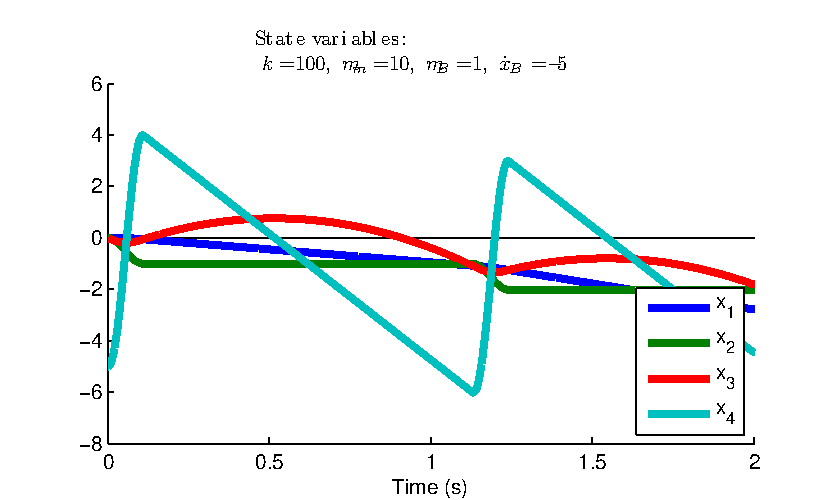
\includegraphics[scale=1]{./images/sys.pdf}
		\caption{	Example simulation for $k=1000$, $m_m=10$, $m_B=1$ and $\dot{x}_B=-5$.}
		\label{fig:SEDA}
	\end{figure}

\subsection{Fixed-point analysis}


%%%%%%%%%%%%%%%%%%%%%%%%%%%%%%%%%%%%%%%%%%%%%%%%%%%%%%%%%%%%%%%%%%%%%%%%%%%%%%%%
\section{Linearized system}


\subsection{Eigenvalue analysis}

%%%%%%%%%%%%%%%%%%%%%%%%%%%%%%%%%%%%%%%%%%%%%%%%%%%%%%%%%%%%%%%%%%%%%%%%%%%%%%%%
\section{LQR Problem}

%TODO: Show min equation
% 		- constraints
%		- 

%%%%%%%%%%%%%%%%%%%%%%%%%%%%%%%%%%%%%%%%%%%%%%%%%%%%%%%%%%%%%%%%%%%%%%%%%%%%%%%%
%\section{Acknowledgments}
%Thanks to early work by Devin Koepl on the spring force math.






\end{document}
